\begin{textbox}{\href{https://compneuro.neuromatch.io/tutorials/W2D2_LinearSystems/student/W2D2_Tutorial1.html}{Linear Dynamical Systems }   }
\begin{subbox}{subbox}{One-dimensional Differential Equations}
\scriptsize
Differential equations are equations that express the \textbf{rate of change} of the state variable $x$. One typically describes this rate of change using the derivative of $x$ with respect to time ($dx/dt$) on the left hand side of the differential equation:

$$\frac{dx}{dt} = f(x)$$

A common notational short-hand is to write $\dot{x}$ for $\frac{dx}{dt}$. The dot means "the derivative with respect to time".
We can simulate an ordinary differential equation by approximating or modeling time as a discrete list of time steps $t_0, t_1, t_2, \dots$, such that $t_{i+1}=t_i+dt$. We can get the small change $dx$ over a small duration $dt$ of time from the definition of the differential:
\begin{eqnarray}
  \dot x &=& \frac{dx}{dt} \\
  dx     &=& \dot x\, dt  
\end{eqnarray}
So, at each time step $t_i$, we compute a value of $x$, $x(t_i)$, as the sum of the value of $x$ at the previous time step, $x(t_{i-1})$ and a small change $dx=\dot x\,dt$:

$$x(t_i)=x(t_{i-1})+\dot x(t_{i-1}) dt$$
This very simple integration scheme, known as \textbf{forward Euler integration}, works well if $dt$ is small and the ordinary differential equation is simple.

The solution of the differential equation $\dot{x} = a x$ using forward Euler integration is: 

\centering
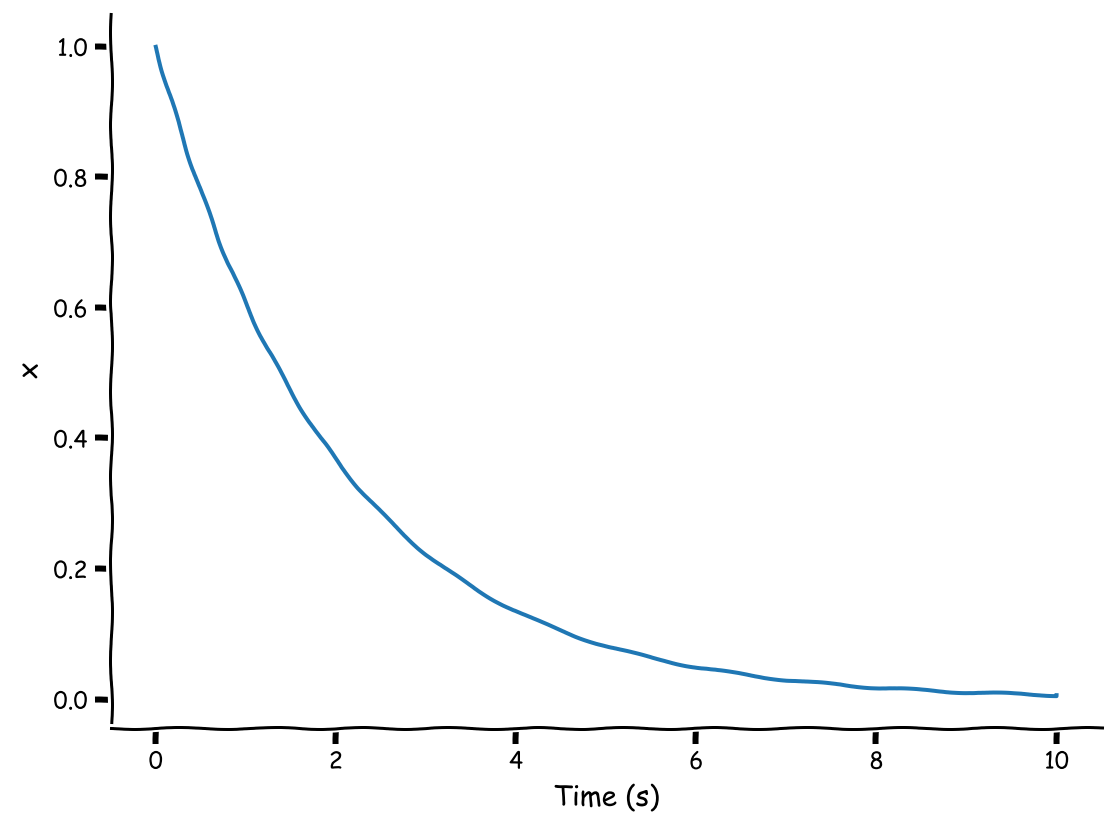
\includegraphics[scale=0.15]{Figures/LS/LSFigure1.png}
\end{subbox}
\end{textbox}
%%%%%%%%%%%%%%%%%%%%%%%%% 
%%%%%%%%%%%%%%%%%%%%%%%%%
\begin{textbox}{\href{https://compneuro.neuromatch.io/tutorials/W2D2_LinearSystems/student/W2D2_Tutorial1.html}{Linear Dynamical Systems } }
\begin{subbox}{subbox}{Multi-Dimensional Dynamics}
\scriptsize
Adding one additional variable (or dimension) adds more variety of behaviors. Additional variables are useful in modeling the dynamics of more complex systems with richer behaviors, such as systems of multiple neurons. We can write such a system using two linear ordinary differential equations:

\begin{eqnarray}
  \dot{x}_1 &=& {a}_{11} x_1 \\
  \dot{x}_2 &=& {a}_{22} x_2 
\end{eqnarray}

So far, this system consists of two variables (e.g. neurons) in isolation. To make things interesting, we can add interaction terms:

\begin{eqnarray}
  \dot{x}_1 &=& {a}_{11} x_1 + {a}_{12} x_2 \\
  \dot{x}_2 &=& {a}_{21} x_1 + {a}_{22} x_2 
\end{eqnarray}

We can write the two equations that describe our system as one (vector-valued) linear ordinary differential equation:

$$\dot{\mathbf{x}} = \mathbf{A} \mathbf{x}$$

For two-dimensional systems, $\mathbf{x}$ is a vector with 2 elements ($x_1$ and $x_2$) and $\mathbf{A}$ is a $2 \times 2$ matrix with 
$$\mathbf{A}=
\begin{pmatrix}
 a_{11} & a_{12} \\
 a_{21} & a_{22} 
\end{pmatrix}.
$$
\centering
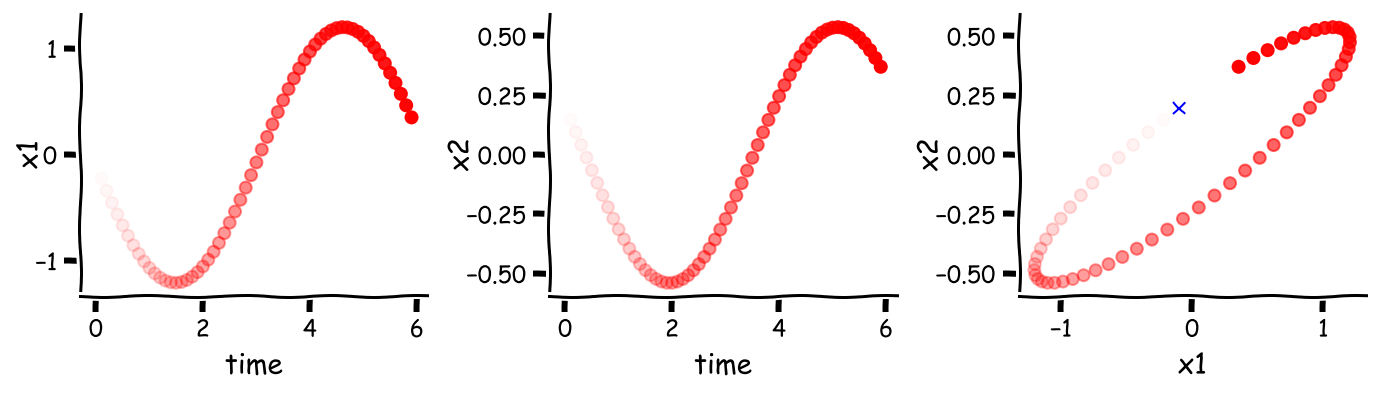
\includegraphics[scale=0.14]{Figures/LS/LSFigure2.png}

\end{subbox}

\end{textbox}
%%%%%%%%%%%%%%%%%%%%%%%%% 
%%%%%%%%%%%%%%%%%%%%%%%%%
\begin{textbox}{\href{https://compneuro.neuromatch.io/tutorials/W2D2_LinearSystems/student/W2D2_Tutorial1.html}{Linear Dynamical Systems } }
\begin{subbox}{subbox}{Stream Plots}
\scriptsize
It's a bit tedious to plot trajectories one initial condition at a time!

Fortunately, to get an overview of how a grid of initial conditions affect trajectories of a system, we can use a \textit{stream plot}. 

We can think of a initial condition ${\bf x}_0=(x_{1_0},x_{2_0})$  as coordinates for a position in a space. For a 2x2 matrix $\bf A$, a stream plot computes at each position $\bf x$ a small arrow that indicates $\bf Ax$ and then connects the small arrows to form \textit{stream lines}. Remember from the beginning of this tutorial that $\dot {\bf x} = \bf Ax$ is the rate of change of $\bf x$. So the stream lines indicate how a system changes. If you are interested in a particular initial condition ${\bf x}_0$, just find the corresponding position in the stream plot. The stream line that goes through that point in the stream plot indicates ${\bf x}(t)$.

Using some helper functions, we show the stream plots for each option of A that you examined in the earlier interactive demo. We included the eigenvectors of $\bf A$ as a red line (1st eigenvalue) and a blue line (2nd eigenvalue) in the stream plots.

\centering
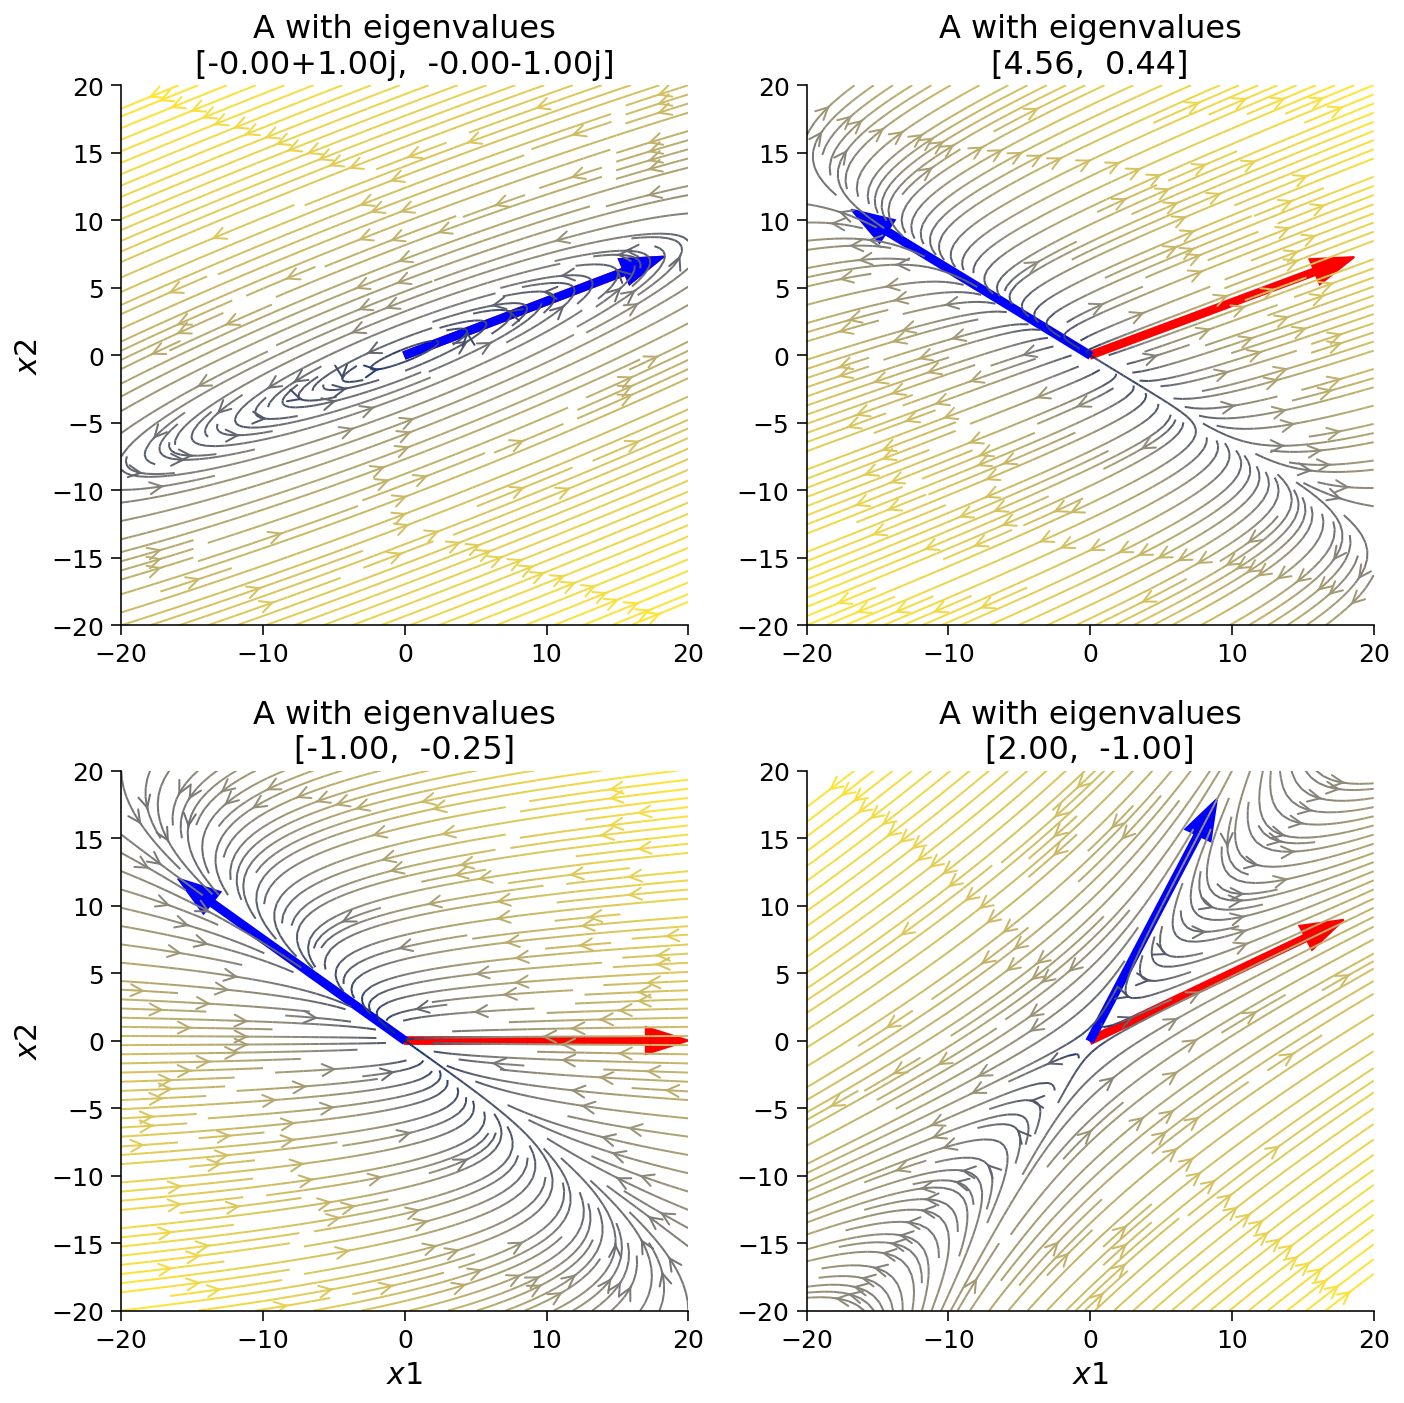
\includegraphics[scale=0.25]{Figures/LS/LSFigure3.png}
\end{subbox}
\end{textbox}
%%%%%%%%%%%%%%%%%%%%%%%%% 
%%%%%%%%%%%%%%%%%%%%%%%%%
\begin{textbox}{\href{https://colab.research.google.com/github/NeuromatchAcademy/course-content/blob/master/tutorials/W2D2_LinearSystems/student/W2D2_Tutorial2.ipynb}{Markov Processes }   }
\begin{subbox}{subbox}{  Introduction }

\scriptsize

We will now look at \textbf{probabilistic} dynamical systems. You may sometimes hear these systems called \textit{stochastic}. In a probabilistic process, elements of randomness are involved. Every time you observe some probabilistic dynamical system, starting from the same initial conditions, the outcome will likely be different. Put another way, dynamical systems that involve probability will incorporate random variations in their behavior. 

For some probabilistic dynamical systems, the differential equations express a relationship between $\dot{x}$ and $x$ at every time $t$, so that the direction of $x$ at every time depends entirely on the value of $x$. Said a different way, knowledge of the value of the state variables $x$ at time t is all the information needed to determine $\dot{x}$ and therefore $x$ at the next time.

This property that the present state entirely determines the transition to the next state  is what defines a \textbf{Markov process} and systems obeying this property can be described as \textbf{Markovian}.


\end{subbox}
\begin{subbox}{subbox}{ Telegraph Process}

\scriptsize

Let's consider a Markov process with two states, where switches between each two states are probabilistic (known as a telegraph process). To be concrete, let's say we are modeling an \textit{ion channel in a neuron that can be in one of two states: Closed (0) or Open (1)}. 

If the ion channel is Closed, it may transition to the Open state with probability $P(0 \rightarrow 1 | x = 0) = \mu_{c2o}$. Likewise, If the ion channel is Open, it transitions to Closed with probability $P(1 \rightarrow 0 | x=1) = \mu_{o2c}$.

We simulate the process of changing states as a Poisson process. The Poisson process is a way to model discrete events where the average time between event occurrences is known but the exact time of some event is not known. Importantly, the Poisson process dictates the following points: 

1. The probability of some event occurring is independent from all other events.

2. The average rate of events within a given time period is constant.

3. Two events cannot occur at the same moment. Our ion channel can either be in an open or closed state, but not both simultaneously. 

In the plot below, we will use the Poisson process to model the state of our ion channel at all points $t$ within the total simulation time $T$. We also track at which times throughout the simulation the state makes a switch. 

\centering
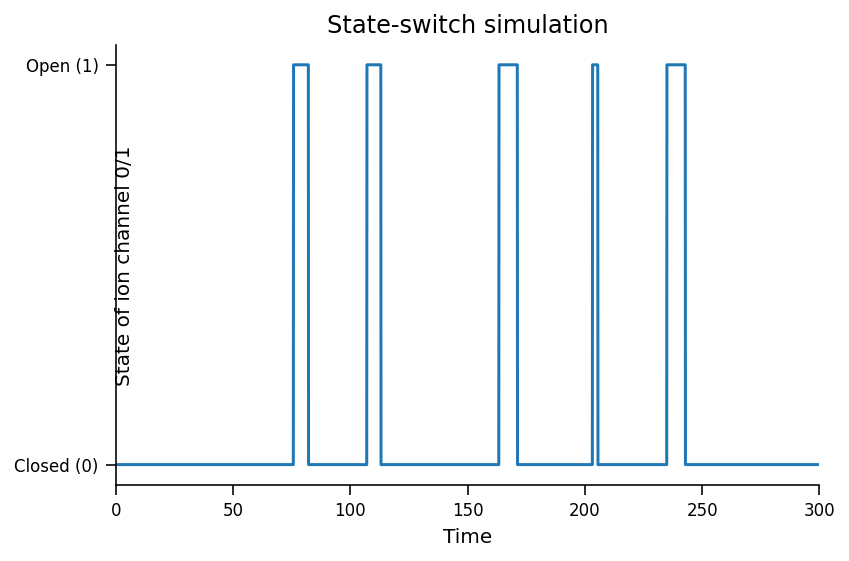
\includegraphics[scale=0.25]{Figures/LS/MC_Figure1.png}

\end{subbox}
\end{textbox}
%%%%%%%%%%%%%%%%%%%%%%%%% 
%%%%%%%%%%%%%%%%%%%%%%%%%
%%%%%%%%%%%%%%%%%%%%%%%%% 
%%%%%%%%%%%%%%%%%%%%%%%%%
\begin{textbox}{\href{https://colab.research.google.com/github/NeuromatchAcademy/course-content/blob/master/tutorials/W2D2_LinearSystems/student/W2D2_Tutorial2.ipynb}{Markov Processes } }
\begin{subbox}{subbox}{Telegraph Process}
\scriptsize

We now have \textit{switch times}, which is a list consisting of times when the state switched. Using this, calculate the time intervals between each state switch and store these in a list called \textit{inter switch intervals}, plotted below.

\begin{center}
    
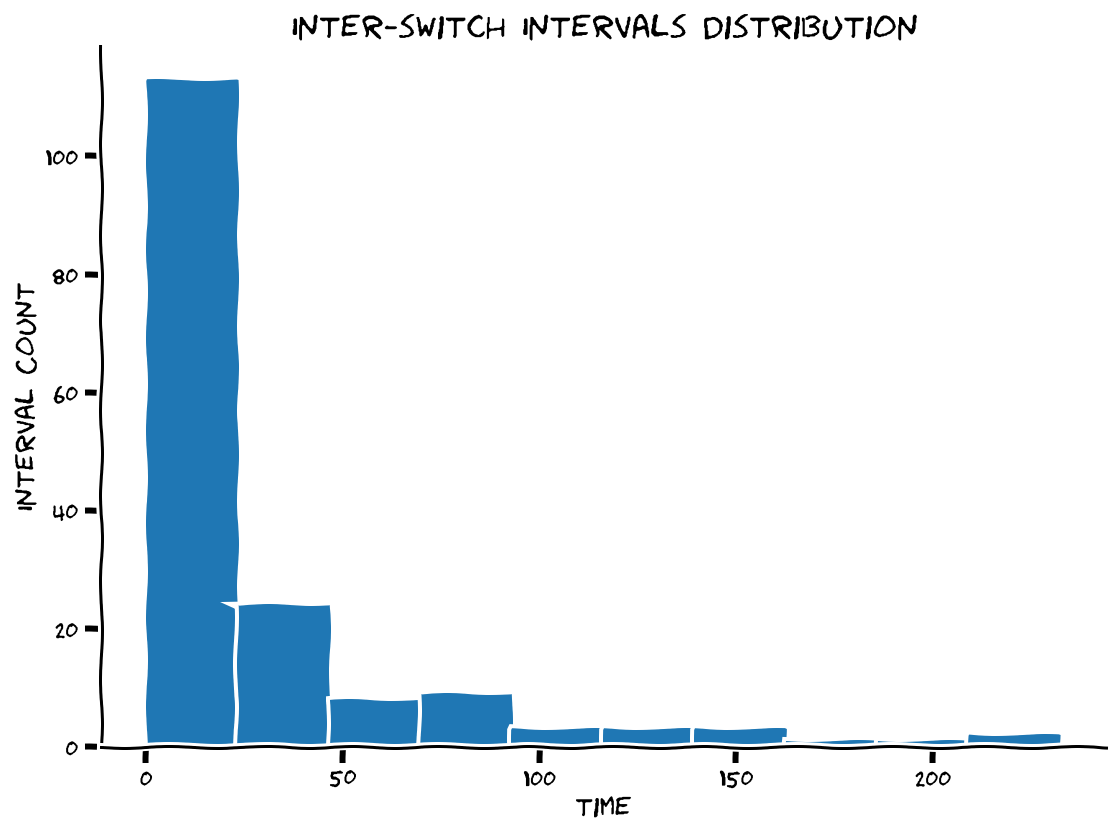
\includegraphics[scale=0.2]{Figures/LS/MC_Figure2.png}
\end{center}

We generate a bar graph to visualize the distribution of the number of time-steps spent in each of the two possible system states during the simulation.
\begin{center}
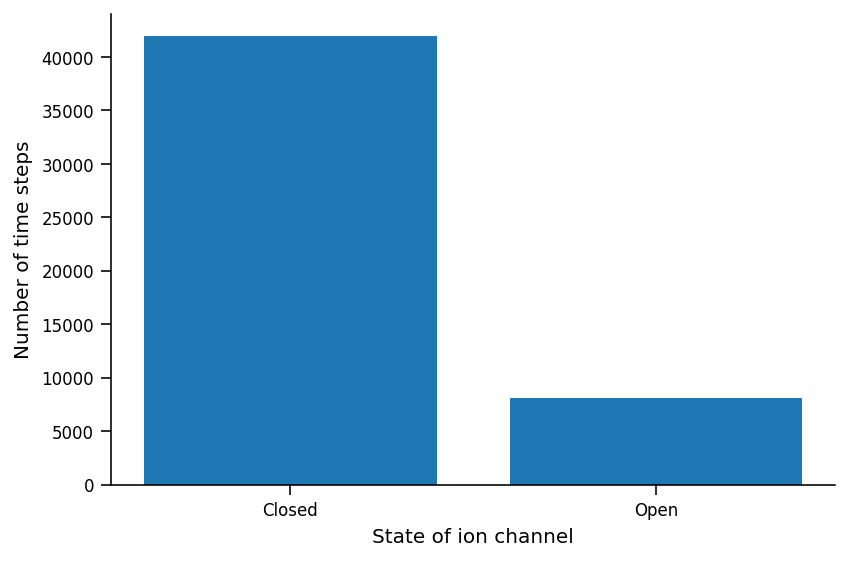
\includegraphics[scale=0.25]{Figures/LS/MC_Figure3.png}
\end{center}

Even though the state is discrete --the ion channel can only be either Closed or Open--we can still look at the \textit{mean state} of the system, averaged over some window of time. 

Since we've coded Closed as $x=0$ and Open as $x=1$, conveniently, the mean of $x$ over some window of time has the interpretation of \textit{fraction of time channel is Open}.

Let's also take a look at the fraction of Open states as a cumulative mean of the state $x$. The cumulative mean tells us the average number of state-changes that the system will have undergone after a certain amount of time. 

\begin{center}
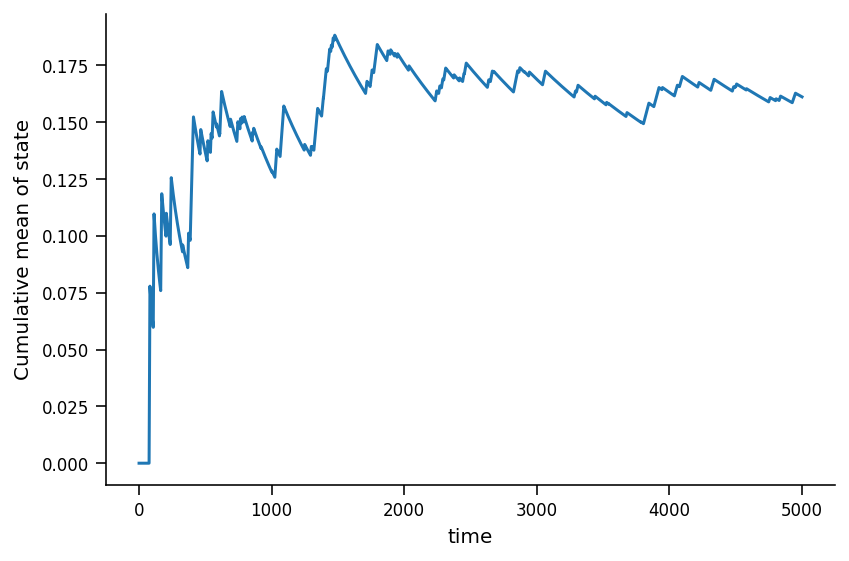
\includegraphics[scale=0.32]{Figures/LS/MC_Figure4.png}
\end{center}
\end{subbox}
\end{textbox}
%%%%%%%%%%%%%%%%%%%%%%%%% 
%%%%%%%%%%%%%%%%%%%%%%%%%
\begin{textbox}{\href{https://colab.research.google.com/github/NeuromatchAcademy/course-content/blob/master/tutorials/W2D2_LinearSystems/student/W2D2_Tutorial2.ipynb}{Markov Processes } }
\begin{subbox}{subbox}{Distributional Perspective}
\scriptsize
We can run a simulation many times and gather empirical distributions of open/closed states. Alternatively, we can formulate the exact same system probabilistically, keeping track of the probability of being in each state.

The same system of transitions can then be formulated using a vector of 2 elements as the state vector and a dynamics matrix $\mathbf{A}$. The result of this formulation is a *state transition matrix*:

\[\left[ \begin{array}{c} C \\ O \end{array} \right]_{k+1} = \mathbf{A} \left[ \begin{array}{c} C \\ O \end{array} \right]_k = \left[ \begin{matrix} 1-\mu_{\text{c2o}} & \mu_{\text{o2c}} \\ \mu_{\text{c2o}} & 1-\mu_{\text{o2c}} \end{matrix} \right] \left[ \begin{array}{c} C \\ O \end{array} \right]_k.\]


Each transition probability shown in the matrix is as follows:
\begin{enumerate}
    \item 
 $1-\mu_{\text{c2o}}$, the probability that the closed state remains closed. 
\item $\mu_{\text{c2o}}$, the probability that the closed state transitions to the open state.
\item  $\mu_{\text{o2c}}$, the probability that the open state transitions to the closed state. 
\item $1-\mu_{\text{o2c}}$, the probability that the open state remains open. 
\end{enumerate}



\textbf{Notice} that this system is written as a discrete step in time, and $\mathbf{A}$ describes the transition, mapping the state from step $k$ to step $k+1$. This is different from what we did in the exercises above where $\mathbf{A}$ had described the function from the state to the time derivative of the state.

\begin{center}
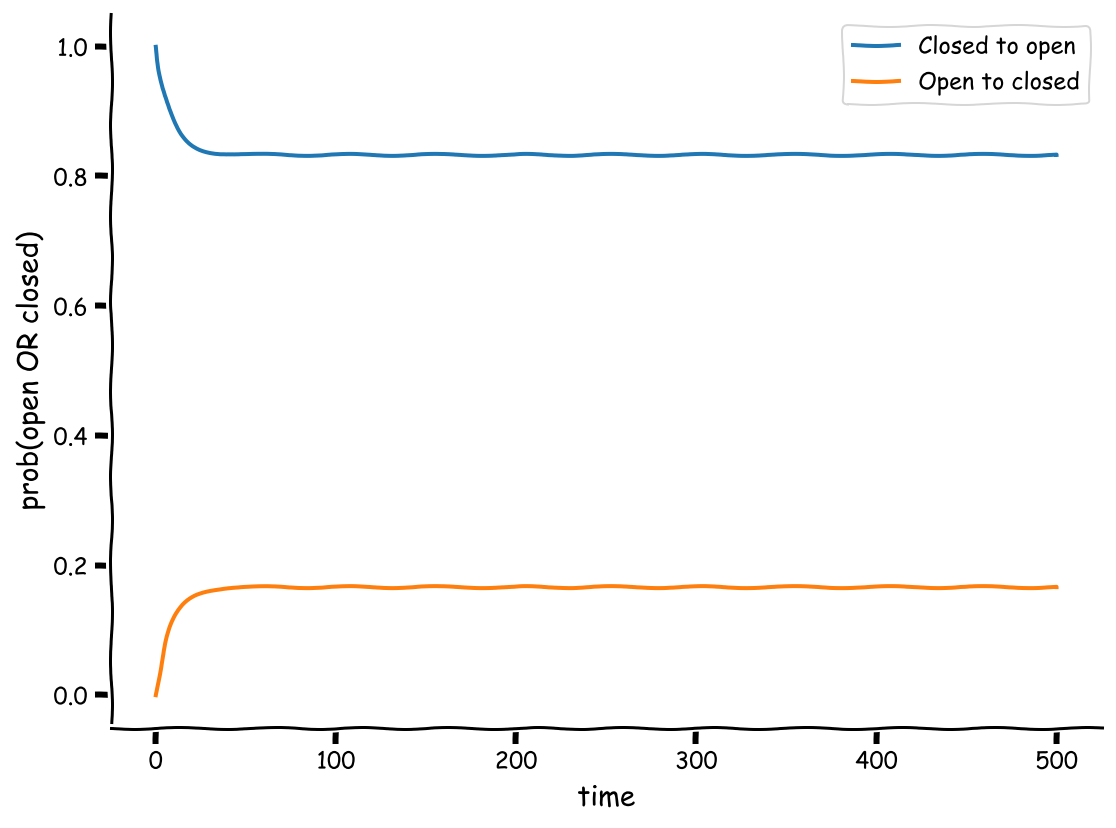
\includegraphics[scale=0.1]{Figures/LS/MC_Figure5.png}
\end{center}

\end{subbox}
\begin{subbox}{subbox}{Equilibrium of the telegraph process}
\scriptsize
Since we have now modeled the propagation of probabilities by the transition matrix $\mathbf{A}$ in Section 2, let's connect the behavior of the system at equilibrium with the eigendecomposition of $\mathbf{A}$.
The eigenvalues of $\mathbf{A}$ tell us about the stability of the system, specifically in the directions of the corresponding eigenvectors.

\end{subbox}
\end{textbox}
%%%%%%%%%%%%%%%%%%%%%%%%% 
%%%%%%%%%%%%%%%%%%%%%%%%%
% Combining determinism and stochasticity
%%%%%%%%%%%%%%%%%%%%%%%%% 
%%%%%%%%%%%%%%%%%%%%%%%%%
\begin{textbox}{\href{https://compneuro.neuromatch.io/tutorials/W2D2_LinearSystems/student/W2D2_Tutorial3.html}{Combining Determinism and Stochasticity } }
\begin{subbox}{subbox}{Introduction}
\scriptsize
We've spent some time familiarizing ourselves with the behavior of such systems when their trajectories are (1) entirely predictable and deterministic, or (2) governed by random processes, it's time to consider that neither is sufficient to describe neuroscience. Instead, we are often faced with processes for which we know some dynamics, but there are some random aspects as well. We call these \textbf{dynamical systems with stochasticity}.

\end{subbox}
\begin{subbox}{subbox}{Random Walks}
\scriptsize
To begin, let's first take a gander at how life sometimes wanders around aimlessly. One of the simplest and best-studied living systems that has some interesting behaviors is the \textit{E. coli} bacterium, which is capable of navigating odor gradients on a substrate to seek a food source. Larger life (including flies, dogs, and blindfolded humans) sometimes use the same strategies to guide their decisions.

Here, we will consider what the \textit{E. coli} does in the absence of food odors. What's the best strategy when one does not know where to head? Why, flail around randomly, of course!

The \textbf{random walk} is exactly that --- at every time step, use a random process like flipping a coin to change one's heading accordingly. Note that this process is closely related to \textbf{Brownian motion}, so you may sometimes hear that terminology used as well.

Let's start with a \textbf{one-dimensional random walk}. A bacterium starts at $x=0$. At every time step, it flips a coin (a very small, microscopic coin of protein mintage), then heads left $\Delta x = -1$ or right $\Delta x = +1$ for with equal probability. For instance, if at time step $1$ the result of the coin flip is to head right, then its position at that time step becomes $x_1 = x_0 + \Delta x = 1.$ Continuing in this way, its position at time step $k+1$ is given by 
$$x_{k+1} = x_k + \Delta x $$    

We will simulate this process below and plot the position of the bacterium as a function of the time step.
\begin{center}
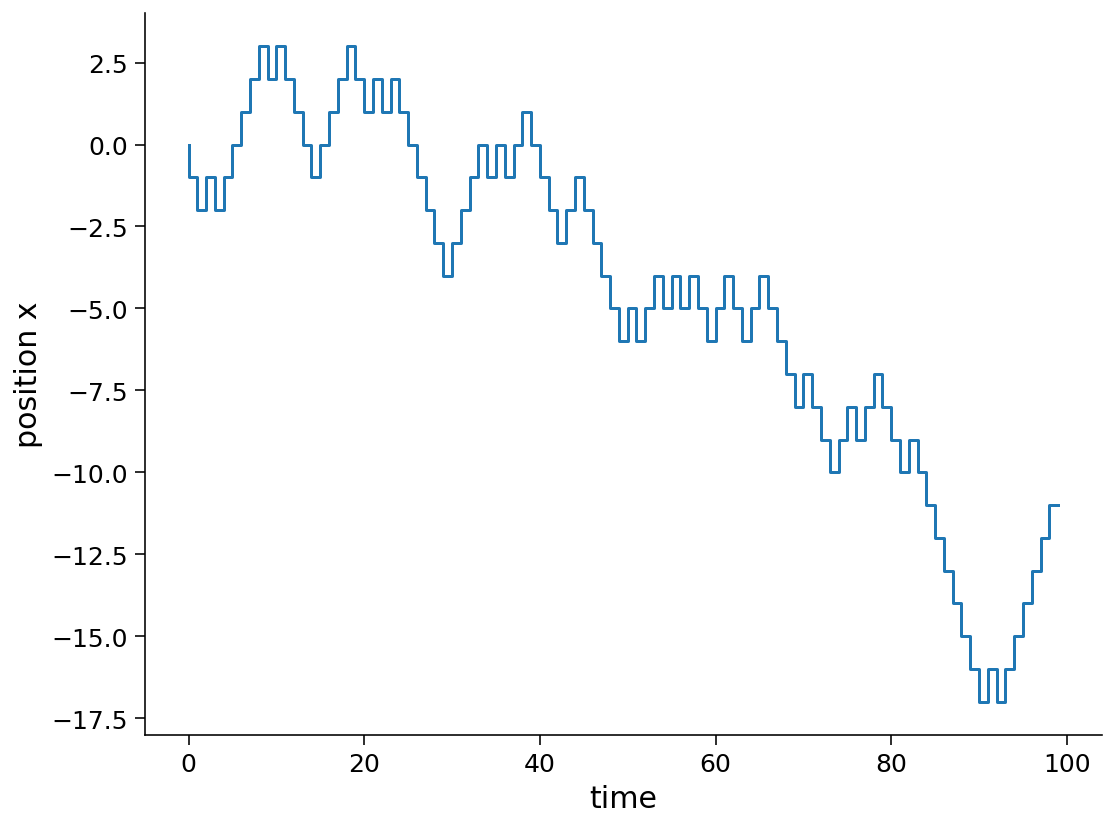
\includegraphics[scale=0.25]{Figures/LS/CDS_Figure1.png}
\end{center}
\end{subbox}
\end{textbox}
%%%%%%%%%%%%%%%%%%%%%%%%% 
%%%%%%%%%%%%%%%%%%%%%%%%%
\begin{textbox}{\href{https://compneuro.neuromatch.io/tutorials/W2D2_LinearSystems/student/W2D2_Tutorial3.html}{Combining Determinism and Stochasticity } }

\begin{subbox}{subbox}{Random Walks Simulations}
\scriptsize
We will plot 10 random walks for 10000 time steps each where the steps have a standard normal distribution (with mean $\mu$ and standard deviation $\sigma$). 


\begin{center}
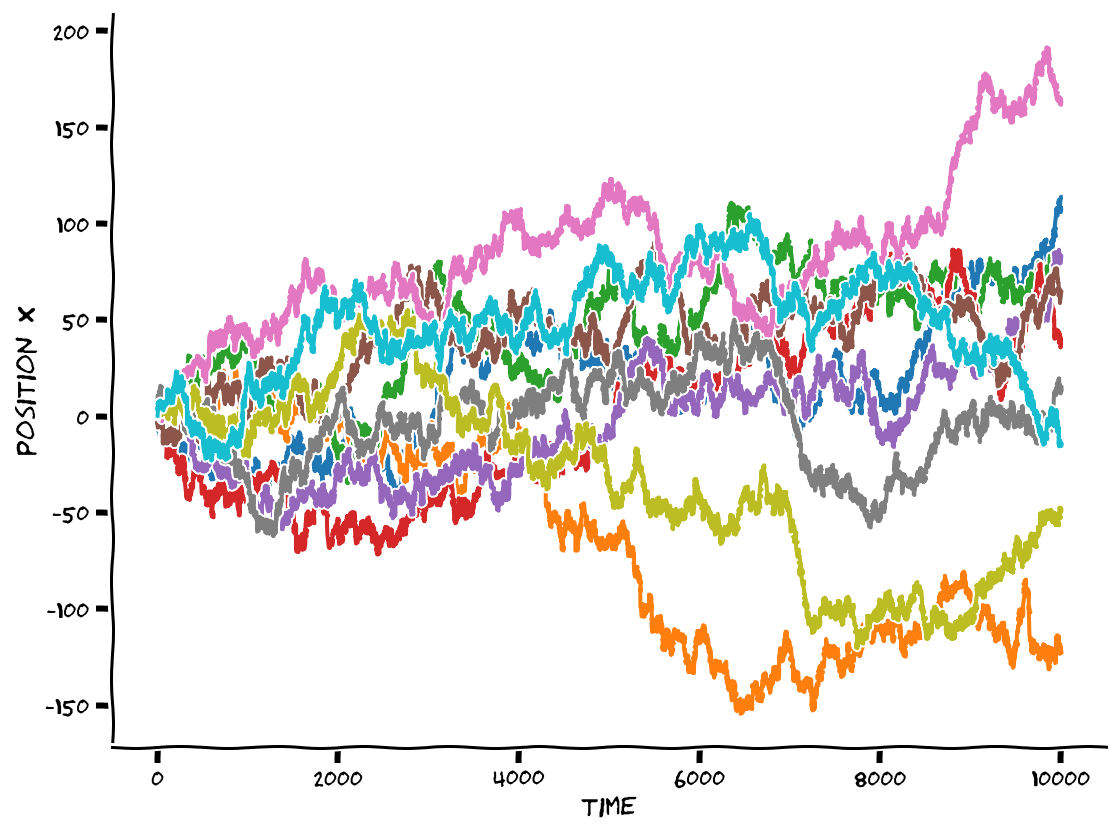
\includegraphics[scale=0.25]{Figures/LS/CDS_Figure3.png}
\end{center}

We see that the trajectories all look a little different from each other. But there are some general observations one can make: at the beginning almost all trajectories are very close to $x=0$, which is where our bacterium started. As time progresses, some trajectories move further and further away from the starting point. However, a lot of trajectories stay close to the starting point of $x=0$. 

Now let's take a look in the next cell at the distribution of bacteria positions at different points in time, analyzing all the trajectories from above.
\begin{center}
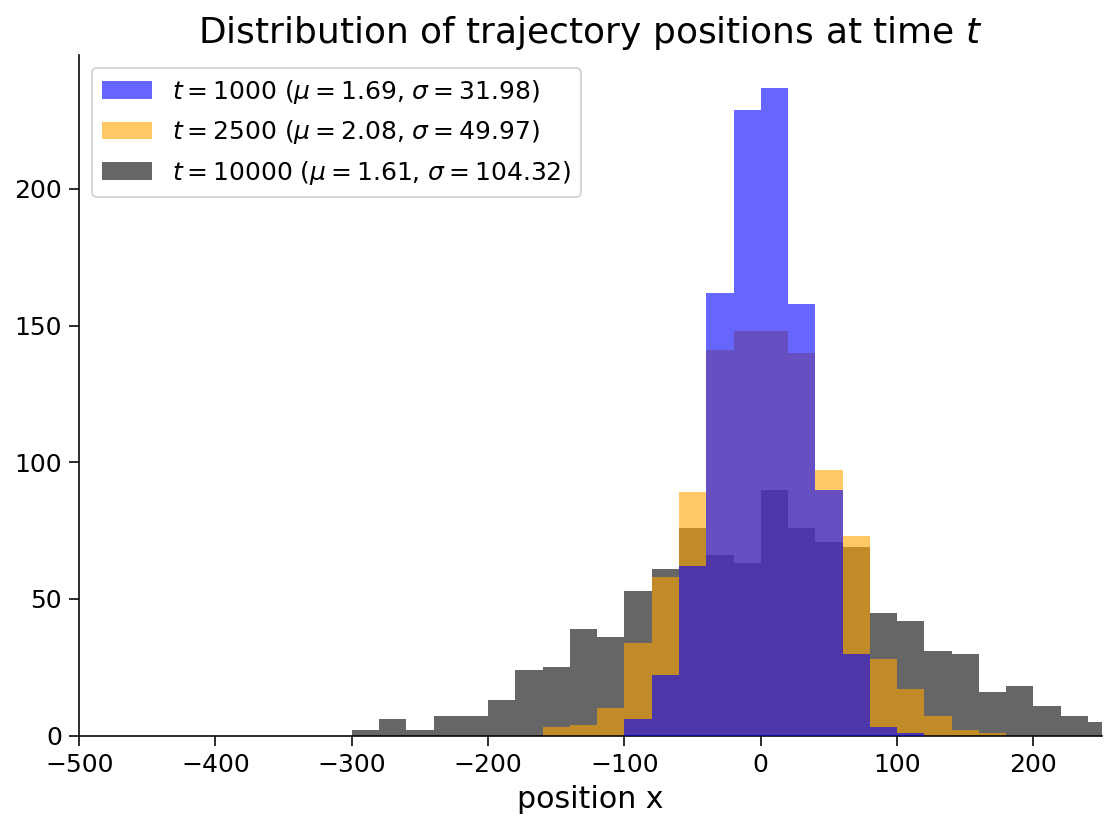
\includegraphics[scale=0.25]{Figures/LS/CDS_Figure4.png}
\end{center}
The plot of the mean and variance of our bacterium's random walk as a function of time.

\begin{center}
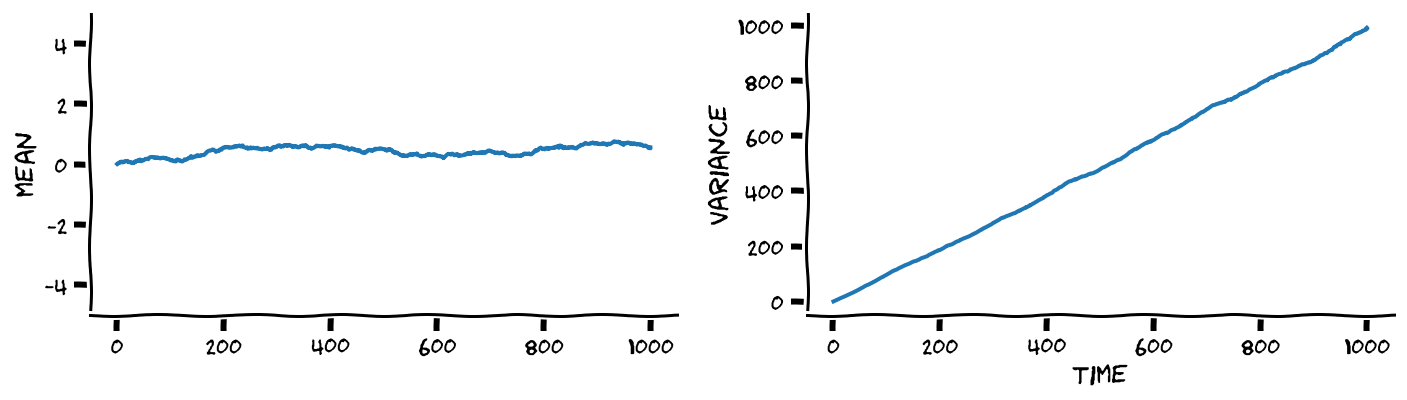
\includegraphics[scale=0.25]{Figures/LS/CDS_Figure5.png}
\end{center}
\end{subbox}
\end{textbox}

%%%%%%%%%%%%%%%%%%%%%%%%% 
%%%%%%%%%%%%%%%%%%%%%%%%%
\begin{textbox}{\href{https://compneuro.neuromatch.io/tutorials/W2D2_LinearSystems/student/W2D2_Tutorial3.html}{Combining Determinism and Stochasticity } }

\begin{subbox}{subbox}{The Ornstein-Uhlenbeck (OU) process}
\scriptsize
Our goal is now to build on this model to construct a \textbf{drift-diffusion} model (DDM). DDM is a popular model for memory, which as we all know, is often an exercise in hanging on to a value imperfectly. Decision-making and memory will be the topic for tomorrow, so here we build the mathematical foundations and develop some intuition for how such systems behave!

To build such a model, let's combine the random walk model with the first order discrete differential equation. We have to modify our analytic solution of the differential equation slightly:

\[x_k = x_\infty(1 - \lambda^k) + x_0 \lambda^k.\]

The dynamics of this process starts at $x_0$ and decay towards $x_{\infty}.$

Now we are ready to take this basic, deterministic difference equation and add a diffusion process on top of it!

As a point of terminology: this type of process is commonly known as a \textbf{drift-diffusion model} or \textbf{Ornstein-Uhlenbeck (OU) process}. The model is a combination of a drift term toward $x_{\infty}$ and a diffusion term that walks randomly. You may sometimes see them written as continuous stochastic differential equations, but here we are doing the discrete version to maintain continuity in the tutorial. The discrete version of our OU process has the following form:

\[x_{k+1} = x_\infty + \lambda(x_k - x_{\infty}) + \sigma \eta\]

where $\eta$ is sampled from a standard normal distribution ($\mu=0, \sigma=1$). 
\begin{center}
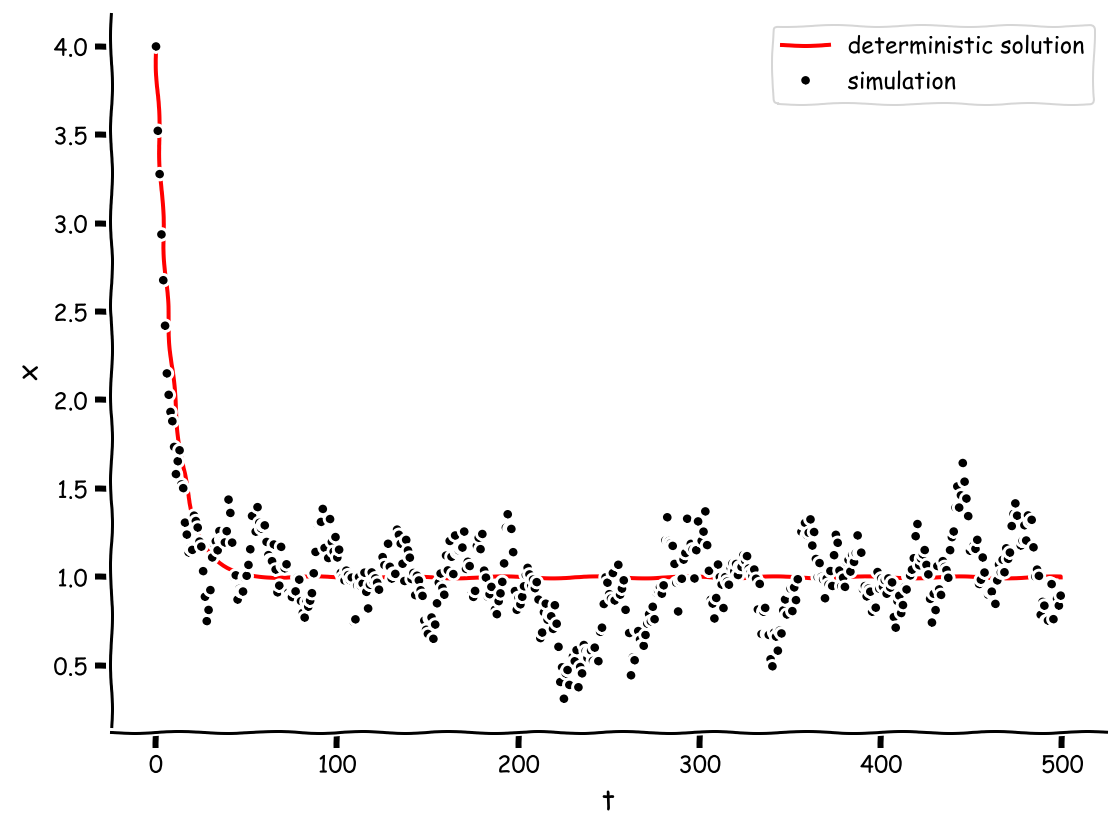
\includegraphics[scale=0.08]{Figures/LS/CDS_Figure7.png}
\end{center}
\end{subbox}
\begin{subbox}{subbox}{Variance of the OU process}
\scriptsize

As we can see, the \textit{mean} of the process follows the solution to the deterministic part of the governing equation. But what about the \texit{variance}? 

Unlike the random walk, because there's a decay process that "pulls" $x$ back towards $x_\infty$, the variance does not grow without bound with large $t$. Instead, when it gets far from $x_\infty$, the position of $x$ is restored, until an equilibrium is reached.

The equilibrium variance for our drift-diffusion system is

\[\text{Var} = \frac{\sigma^2}{1 - \lambda^2}.\]

Notice that the value of this equilibrium variance depends on $\lambda$ and $\sigma$. It does not depend on $x_0$ and $x_\infty$.

\end{subbox}

\end{textbox}
%%%%%%%%%%%%%%%%%%%%%%%%% 
%%%%%%%%%%%%%%%%%%%%%%%%%
%%% Autoregressive models
%%%%%%%%%%%%%%%%%%%%%%%%% 
%%%%%%%%%%%%%%%%%%%%%%%%%
\begin{textbox}{\href{https://compneuro.neuromatch.io/tutorials/W2D2_LinearSystems/student/W2D2_Tutorial4.html}{Autoregressive models } }
\begin{subbox}{subbox}{Fitting data to the OU process}
\scriptsize
 Our process  the drift-diffusion (OU) process had following form:
\[x_{k+1} = x_{\infty} + \lambda(x_k - x_{\infty}) + \sigma \eta\]
where $\eta$ is sampled from a standard normal distribution. 
For simplicity, we set $x_\infty = 0$. Let's plot a trajectory for this process again below. Take note of the parameters of the process because they will be important later.

\begin{center}
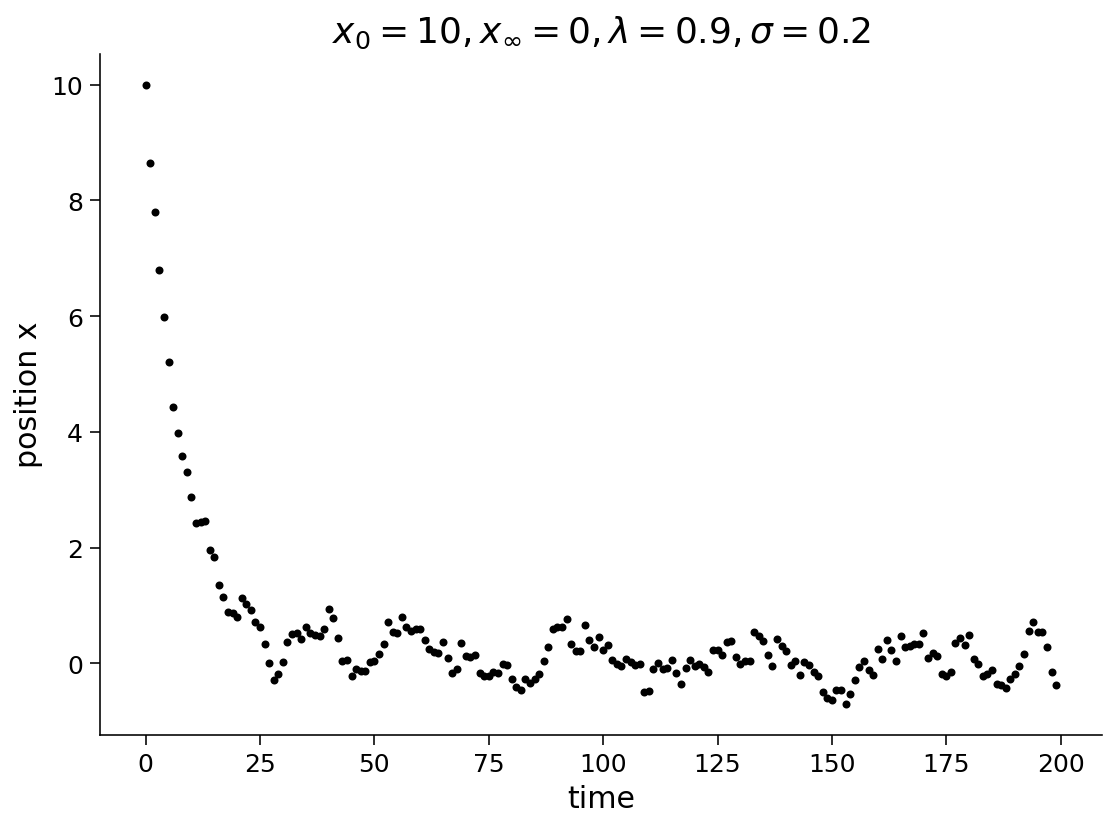
\includegraphics[scale=0.25]{Figures/LS/CDS_Figure8.png}
\end{center}
What if we were given these positions $x$ as they evolve in time as data, how would we get back out the dynamics of the system $\lambda$? 

Since a little bird told us that this system takes on the form

$$x_{k+1} = \lambda x_k + \eta,$$

where $\eta$ is noise from a normal distribution, our approach is to solve for $\lambda$ as a \textbf{regression problem}. 

As a check, let's plot every pair of points adjacent in time ($x_{k+1}$ vs. $x_k$) against each other to see if there is a linear relationship between them. 

Hooray, it's a line! This is evidence that the dynamics that generated the data is linear. We can now reformulate this task as a regression problem.
\begin{center}
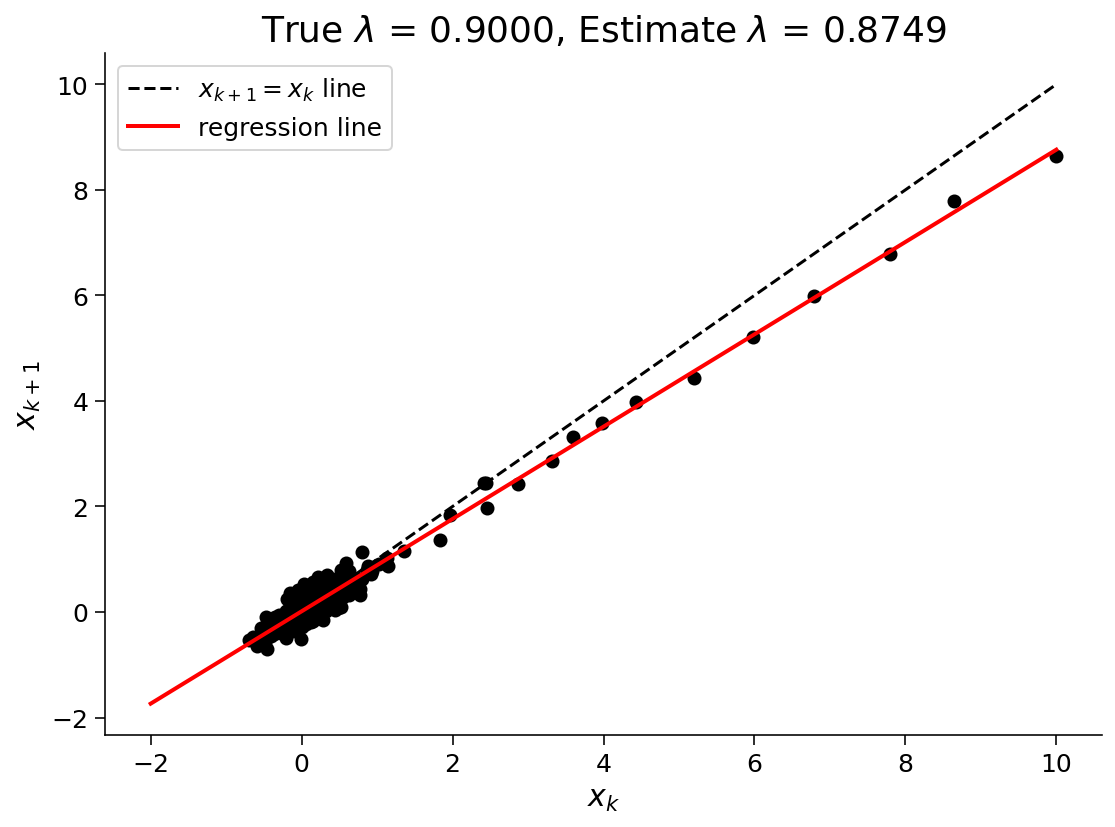
\includegraphics[scale=0.25]{Figures/LS/CDS_Figure10.png}
\end{center}
This model is \textbf{autoregressive}, where auto means self. In other words, it's a regression of the time series on itself from the past. The equation as written above is only a function of itself from one step in the past, so we can call it a first order autoregressive model and plot.


\end{subbox}

\end{textbox}
%%%%%%%%%%%%%%%%%%%%%%%%% 
%%%%%%%%%%%%%%%%%%%%%%%%%
\begin{textbox}{\href{https://compneuro.neuromatch.io/tutorials/W2D2_LinearSystems/student/W2D2_Tutorial4.html}{Autoregressive models } }
\begin{subbox}{subbox}{Higher order autoregressive models}
\scriptsize
Now that we have established the autoregressive framework, generalizing for dependence on data points from the past is straightforward. \textbf{Higher order} autoregression models a future time point based on more than one point in the past.

In one dimension, we can write such an order-$r$ model as
$$
x_{k+1} = \alpha_0 + \alpha_1 x_k + \alpha_2 x_{k-1} + \alpha_3 x_{k-2} + \dots + \alpha_{r+1} x_{k-r} \text{  , }
$$
where the $\alpha$'s are the $r+1$ coefficients to be fit to the data available.

These models are useful to account for some \textbf{history dependence} in the trajectory of time series. This next part of the tutorial will explore one such time series, and you can do an experiment on yourself!

In particular, we will explore a binary random sequence of 0's and 1's that would occur if you flipped a coin and jotted down the flips. 

The difference is that, instead of actually flipping a coin (or using code to generate such a sequence), you -- yes you, human -- are going to generate such a random Bernoulli sequence as best as you can by typing in 0's and 1's. We will then build higher-order AR models to see if we can identify predictable patterns in the time-history of digits you generate.
\begin{center}
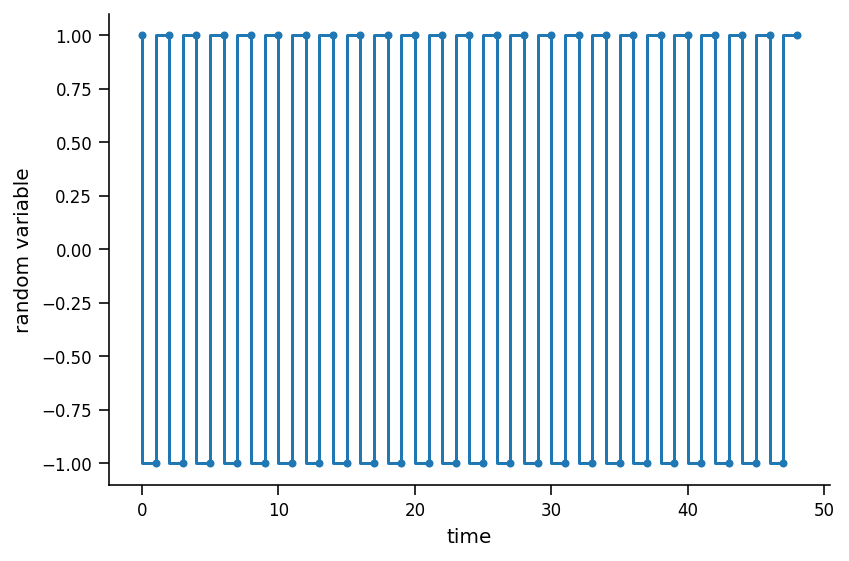
\includegraphics[scale=0.4]{Figures/LS/CDS_Figure11.png}
\end{center}

\end{subbox}

\end{textbox}

%%%%%%%%%%%%%%%%%%%%%%%%% 
%%%%%%%%%%%%%%%%%%%%%%%%%
\begin{textbox}{\href{https://compneuro.neuromatch.io/tutorials/W2D2_LinearSystems/student/W2D2_Tutorial4.html}{Autoregressive models } }

\begin{subbox}{subbox}{Understanding autoregressive parameters}
\scriptsize
Truly random sequences of numbers have no structure and should not be predictable by an AR or any other models.

However, humans are notoriously terrible at generating random sequences of numbers! (Other animals are no better...)

To test out an application of higher-order AR models, let's use them to model a sequence of 0's and 1's that a human tried to produce at random. 

If the digits really have no structure, then we expect our model to do about as well as guessing, producing an error rate of 0.5. Let's see how well we can do!

Fit a order-5 ($r=5$) AR model to the data vector $x$. We will then plot the observations against the trained model. Note that this means we are using a sequence of the previous 5 digits to predict the next one. 

Additionally, output from our regression model is continuous (real numbers) whereas our data are scalar (+1/-1). So, we will take the sign of our continuous outputs (+1 if positive and -1 if negative) as our predictions to make them comparable with data. Our error rate will simply be the number of mismatched predictions divided by the total number of predictions.
\begin{center}
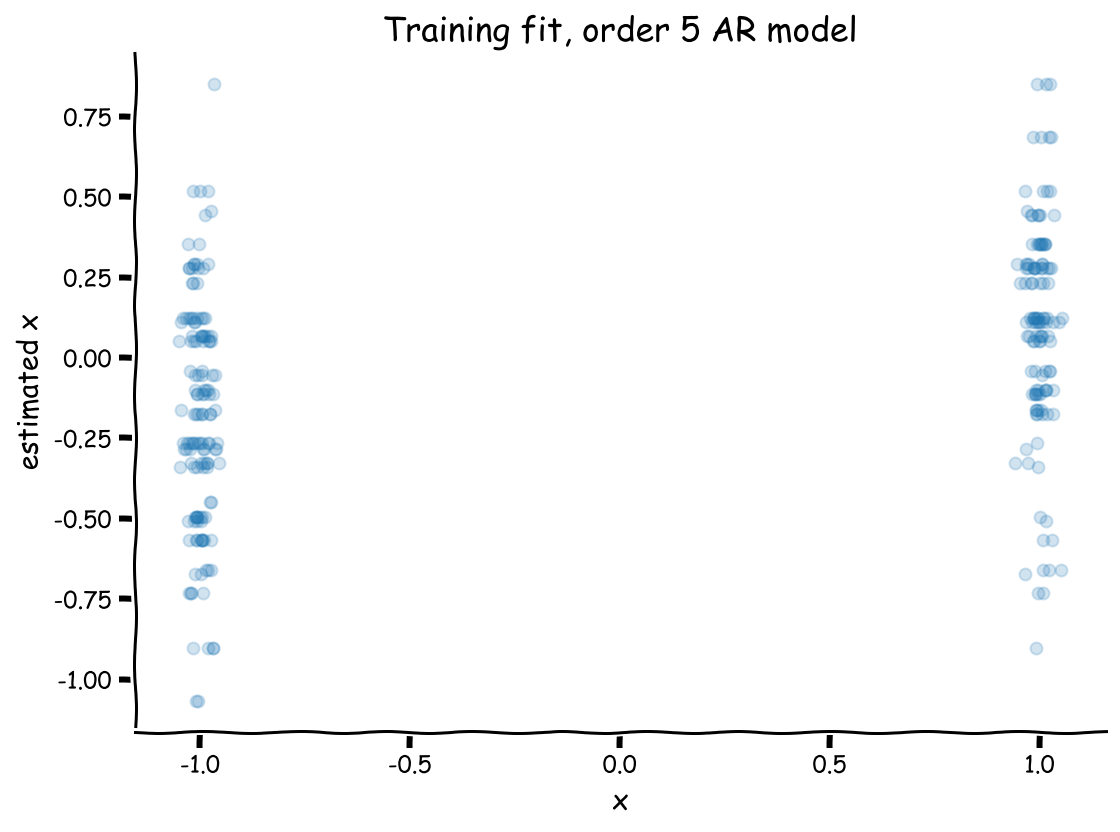
\includegraphics[scale=0.15]{Figures/LS/CDS_Figure12.png}
\end{center}
Let's now try \textbf{AR models of different orders} systematically, and plot the test error of each.

\begin{center}
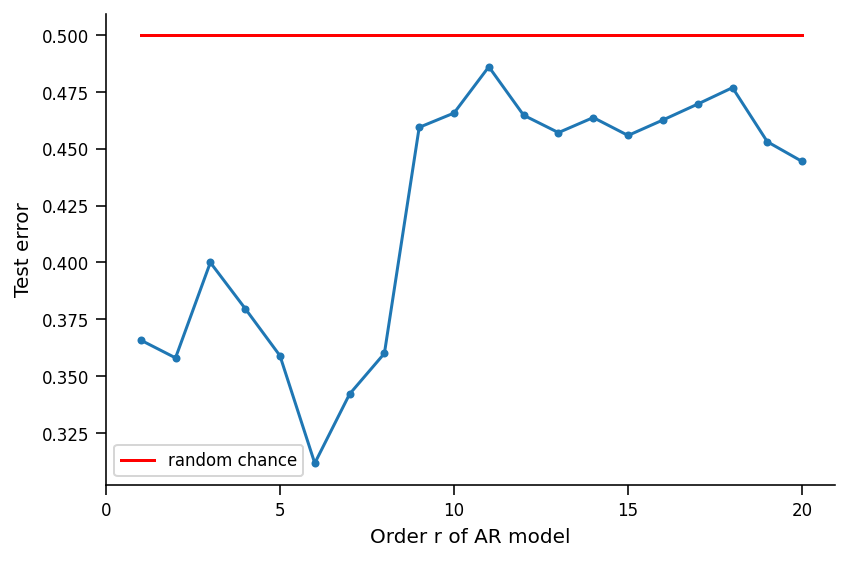
\includegraphics[scale=0.35]{Figures/LS/CDS_Figure13.png}
\end{center}


Notice that there's a sweet spot in the test error! The 6th order AR model does a really good job here, and for larger $r$'s, the model starts to overfit the training data and does not do well on the test data.

\end{subbox}
\end{textbox}